\usetikzlibrary {angles, quotes}
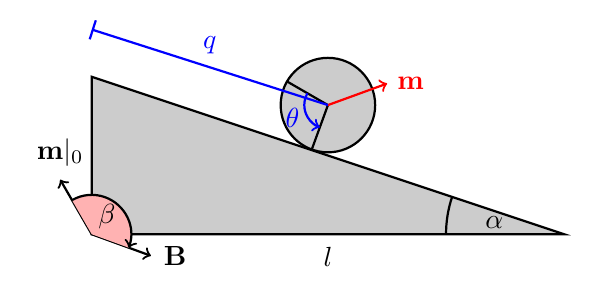
\begin{tikzpicture}[scale=.4]
    \coordinate (A) at (0,5);
    \coordinate (B) at (0,0);
    \coordinate (C) at (15,0);
    \coordinate (D) at (7.5, 4.1);
    \filldraw[thick, fill=black!20] (A) -- (B) -- node[midway, below=1] {$l$} (C) -- cycle
        pic [draw=black, angle radius=15mm, "$\alpha$"] {angle = A--C--B};
    \filldraw[thick, fill=black!20] (7.5, 4.1) circle [radius=1.5];
    \draw[thick]  (D)+(150:1.5) coordinate (F) -- (D) -- +(250:1.5) coordinate (G)
    pic [draw=blue, angle radius=3mm, "\textcolor{blue}{$\theta$}", angle eccentricity =1.6, ->] {angle = F--D--G};
    \draw[thick, red, ->] (D) -- +(20:2) coordinate[ label=right:\textcolor{red}{$\mathbf{m}$}] (H);  
    %\pic[thick, draw=red, angle radius=3mm, "\textcolor{red}{$\beta$}", angle eccentricity=1.6] {angle = H--D--F};
    \draw[thick, blue, |-]  (A)+(0,1.5) -- node[above=1, midway] {$q$} (D);
    \draw[thick, black, ->] (B) -- (340:2) coordinate (B1) node[right=1] {$\mathbf{B}$};
    \draw[thick, black, ->] (B) -- (120:2) coordinate (B2) node[above=1] {$\mathbf{m}|_0$};
    \pic[thick, draw=black, fill=red!30, angle radius=5mm, "$\beta$", <-] {angle = B1--B--B2};
\end{tikzpicture}
